% -----------------------------------------------
% Template for ISMIR 2014
% (based on earlier ISMIR templates)
% -----------------------------------------------

\documentclass{article}
\usepackage{ismir2014,amsmath,cite}
\usepackage{graphicx}
\usepackage{multirow}
\usepackage{units}

% Title.
% ------
\title{DRUM TRANSCRIPTION IN POLYPHONIC MUSIC USING SEMI-SUPERVISED NON-NEGATIVE MATRIX FACTORIZATION}

% Single address
% To use with only one author or several with the same address
% ---------------
%\oneauthor
% {Names should be omitted for double-blind reviewing}
% {Affiliations should be omitted for double-blind reviewing}

% Two addresses
% --------------
%\twoauthors
%  {First author} {School \\ Department}
%  {Second author} {Company \\ Address}

% Three addresses
% --------------
\threeauthors
  {First author} {Affiliation1 \\ {\tt author1@ismir.edu}}
  {Second author} {\bf Retain these fake authors in\\\bf submission to preserve the formatting}
  {Third author} {Affiliation3 \\ {\tt author3@ismir.edu}}

% Four addresses
% --------------
%\fourauthors
%  {First author} {Affiliation1 \\ {\tt author1@ismir.edu}}
%  {Second author}{Affiliation2 \\ {\tt author2@ismir.edu}}
%  {Third author} {Affiliation3 \\ {\tt author3@ismir.edu}}
%  {Fourth author} {Affiliation4 \\ {\tt author4@ismir.edu}}

\begin{document}
%
\maketitle
%
\begin{abstract}
In this paper, a drum transcription algorithm using semi-supervised non-negative matrix factorization has been presented. This method allows users to separate percussive activities from harmonic activities with pre-trained drum templates, and detect drum events from the extracted percussive activity matrix. A polyphonic subset from ENST drum data set has been used for training and testing of the algorithm. The system has been tested using different rank settings, and a cross-performer validation process has been performed to evaluate the reliability of the system.  The results show that the system can achieve 61 to 77\% recognition rate on multiple drums in polyphonic music. In the future, more efforts will be put on differentiating different playing styles and more drum parts, leading toward a complete drum transcription system.

\end{abstract}
%

\section{Introduction}\label{sec:introduction}
Automatic music transcription is one of the most intensively researched areas in Music Information Retrieval (MIR). The reliable extraction of a score (or a score-related representation) from the audio signal will be the core technology of a large number of applications in fields such as music education, systematic musicology, and music visualization. Furthermore, a reliable transcription would enable high-level representations of music signals with the potential of improving virtually any MIR task.

%Transcribing music content into sheet music or any form of score is an essential skill to musicians for analysis and composition purposes. However, It is often considered a time-consuming and non-trivial task, for it requires repetitive listening and integral knowledge of music and instruments. With the advance of computing power and various machine learning techniques, a system that has the abilities to automatically recognize music content has become a plausible idea and interests many researchers in the field of Music Information Retrieval (MIR) \cite{1}. In general, Automatic Music Transcription (AMT) systems could not only serve as a tool to record the music content, identify notes from improvisations, but also lead to the realization of a music intelligence system \cite{2}. To build a complete AMT system, many subtasks and challenges, such as multi-pitch detection, onset detection, instrument recognition, and rhythm extraction, have been attempted [1]. Comparing with pitched instruments, transcribing un-pitched music events such as percussive sounds seem to be less addressed, and a robust algorithm to detect drum sounds in polyphonic music is still an open question in this field.

%WHAT IS CITATION [2]? A: just a reference to make my point on intellegence music system. Removed

A complete transcription system comprises many related sub-tasks such as multi-pitch detection, onset detection, instrument recognition, and rhythm extraction \cite{Benetos2013}. While the main focus is mostly on pitched instruments, a considerable amount of publications deal with the transcription of percussive sounds in polyphonic music. The drum track in popular music conveys information about tempo, rhythm, style, and possibly the structure of a song. A drum transcription system alone enables applications in music production \cite{Yoshii2007a}, music education, and interactive music performance \cite{Weinberg2009}.

%Drum track, especially in pop music, often plays an important role in determining music structure, style, rhythm and tempo. In many cases, it shares the same importance as the harmonic part in the music. That said, a good drum transcription system could provide essential information of the music content, and could potentially facilitate the realization of many interesting applications. For example, a drum transcription and drum source separation task could mutually benefit from each other and provide the possibility to manipulate drum sounds within an existing drum track \cite{3,4}.  Also, music education could be an application of a drum transcription system, for it could help students identify drum event within a polyphonic music, and provide instructions by analyzing and comparing the differences between the input and reference performances. Furthermore, such system could also be integrated as a part of machine listening, improving the existing systems of robotic musicians \cite{5}.

This study explores the application of the popular transcription method of Non-Negative Matrix Factorization (NMF) for drum transcription in polyphonic music. The paper is structured as follows: Section~\ref{sec:related works} provides an overview of the research in this area. In Sect.~\ref{sec:method} we present our approach; evaluation results are being presented and discussed in Sect.~\ref{evaluation}. Section~\ref{conclusion} provides a summary, conclusion, and directions of future work.

%Therefore, this study aims to explore alternative solutions to drum transcription in polyphonic music. The final goal of this paper is to find a potential direction to push the limit of this task, leading toward further musical applications.

\section{Related Work}\label{sec:related works}
WITHOUT HAVING THE PAPERS I CANNOT REVIEW THIS SECTION --- SKIPPED FOR NOW!

The early attempts to transcribe percussive sounds main focused on classifying monophonic signals \cite{Herrera2002}    \cite{Society2003}. With standard approaches such as feature extraction and classification, fairly high accuracy were reported in the previous studies. However, in the real use case, a drum transcription system is expected to work in polyphonic signal instead of monophonic. Therefore, solving this problem in the context of polyphonic music had become another criterion, and different methods could be found in previous research \cite{FitzGerald2003}\cite{Yoshii2004b}\cite{Dittmar2012}\cite{Dittmar2005}\cite{Tanghe2005b}\cite{Gillet2008}.  According to \cite{Gillet2008}, recent studies on the drum transcription in polyphonic music could be categorized into three types: segment and classify, separate and detect, match and adapt.  For the first type of approaches, the common procedure starts by applying onset detection to the audio signal in order to segment the music event. Once the event has been detected, various features from time or spectral domain of the signal will be extracted, and a classifier will be trained to classify the event based on the extracted features. This type of approaches seem to perform well when the data and features are well chosen \cite{Tanghe2005b}\cite{Alves2009}. However, to get good results, sufficient amount of data, careful preprocessing and training steps are required in this type of systems. Additionally, to handle the situation of simultaneous sounds, more classes need to be trained.

The second type of approaches is based on the assumption that music signal is a superposition of different sound sources. By decomposing the signal and into different source templates and corresponding activities, the music content could be transcribed by detecting onsets of these activities. Different methods such as Independent Subspace Analysis (ISA) \cite{FitzGerald2002}, Prior Subspace Analysis (PSA) \cite{FitzGerald2003}, and Non-negative Matrix Factorization (NMF) \cite{Alves2009}\cite{Paulus2005}\cite{Moreau2007} are the examples in this category. This type of approaches is usually easier to interpret, since most of the decompositions have been done on the spectrogram of the signal. Also, the separate nature allows simultaneous events to be handled easily in this case. However, to be able to transcribe different kinds of music, a large template might be required prior to the decomposition. Moreover, the number of rank during the decomposition process could be difficult to determine in some cases. 

The third type of approaches uses pre-trained templates to detect drum events \cite{Yoshii2007}. An iterative process has been taken to search for the closest matches to these templates and adapt them. The proposed system has been evaluated and performed well in MIREX 2005 drum detection competition. However, to coverage a wider range of sounds, multiple seed templates need to be prepared prior to the process.

In this paper, a method based on the NMF approach has been presented. Although NMF has been proven to be effective in music transcription (\cite{Smaragdis2003}), it is still difficult to determine the number of sources in the target signal for a correct rank parameter setting. Therefore, the goal of this paper is to develop an algorithm that provides a more general use case, which only requires users to input a few drum samples prior to the decomposition process. This method aims to serve as an alternative way to transcribe drum tracks in polyphonic music, leading toward an end user application for general drum transcription tasks.  
 
\section{Method}\label{sec:method}
\subsection{Algorithm Description}\label{subsec:algorithm description}
% introduce NMF here
The basic concept of NMF is to approximate a non-negative matrix $V$ with two non-negative matrices $W$ and $H$ as shown in Eq.~\eqref{eq:approx}.

% equation here
\begin{equation}
V \approx WH
\label{eq:approx}
\end{equation}

That is, given a $m \times n$ matrix $V$, the NMF will decompose the matrix into the product of a $m \times r$ matrix $W$ and a $r \times n$ matrix $H$, with $r$ being the rank of the NMF decomposition. $W$ is the dictionary matrix, and $H$ is the activation matrix. In most audio applications, $V$ is the spectrogram to be decomposed, $W$ contains the magnitude spectra of the salient components, and $H$ indicates the activation of these components with respect to time. The matrices $W$ and $H$ are obtained through an iterative process that minimizes a distance measure between the target spectrogram $V$ and its approximation. \cite{Seung2001}. 

The application of this method to music transcription, however, offers some challenges. 
First, the number of sound sources and notes within a music recording is usually unknown. It is therefore difficult to estimate a correct rank number and obtain a clear representation of the decomposed  components. 
Second, it is hard to identify the corresponding instrument of every component in the dictionary matrix $W$, especially when the rank is very high or very low. 
Third, when multiple similar entries exist in the dictionary matrix, the corresponding activation matrix could be activated at these entries simultaneously and might cause some confusions. %MAYBE THERE IS A POINT TO BE MADE ABOUT THE ACTIVITY MATRIX AS WELL?
Different methods have been proposed in the previous studies to address these issues. Virtanen trained an SVM to separate drum components from the harmonic components; the rank number was derived empirically during the factorization process (\cite{Helen2005}). The identified drum components and their corresponding activities could later be used to reconstruct the drum signal, resulting in a system for drum source separation. Virtanen's approach requires a significant amount of training data for the classifier and, more importantly, the results can be expected to be very susceptible to choice of rank. %However, this method requires separated data to train the classifier, and the results could be data-dependent. 
Yoo proposed a co-factorization algorithm \cite{Yoo2010} to simultaneously factorize a drum track a target signal containing this track and use the basis matrix from the drum track to identify the drum components in the target signal. This method ensures that the drum components in both basis matrices remain the same over the iterations, and thus proper isolation of the harmonic components from the drum components. The need to obtain a drum track prior to the factorization process, however, impacts the usefulness this approach for many application scenarios.

%============= Factorization figure
\begin{figure}
 \centerline{\framebox{
 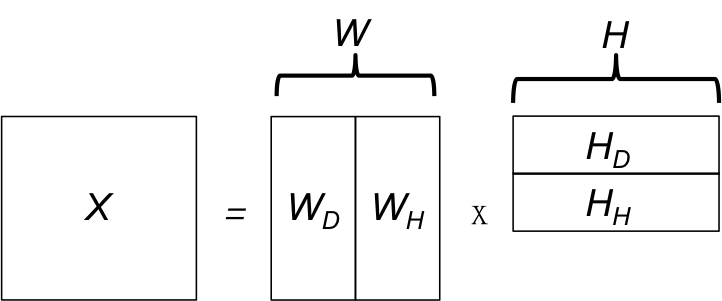
\includegraphics[width=\columnwidth]{factorization.png}}}
 \caption{Illustration of the factorization process. The pre-trained drum basis matrix $W_D$ will not be updated over the iterations.} %WHY IS V CALLED X HERE AND IN THE FOLLOWING EQUATIONS??? 
 \label{fig:factorization}
\end{figure}

% introduce my modification here 
Nevertheless, Yoo's work on co-factorization inspired our work to present a similar system without the requirement the prior drum track. \figref{fig:factorization} visualizes the basic concept: the matrices $W$ and $H$ are split into the  matrices $W_D$ and $W_H$, and  $H_D$ and $H_H$, respectively. 
The matrix $W_D$ is initialized with the drum templates to be detected and will not be updated. Matrices $W_H$, $H_H$, and $H_D$ can be initialized with random numbers. 
The cost function as shown in Eq.~\eqref{eq:costFunc} is minimized by applying gradient decent and multiplicative update rules, the matrices  $W_H$, $H_H$, and $H_D$ will be updated according to Eqs.~\eqref{eq:updateHD}--\eqref{eq:updateHH}.  %\eqref{eq:updateHD} \eqref{eq:updateWH} \eqref{eq:updateHH}.  
% equation here
\begin{equation}
C = \frac{1}{2} || V - W_{D}H_{D} - W_{H}H_{H}||^{2}
\label{eq:costFunc}
\end{equation}

% equation here
\begin{eqnarray}\label{eq1}
H_{D} &\leftarrow& H_{D}\frac{W_{D} ^T V}{W_{D}^T W_{D} H_{D} + W_{D} W_{H} H_{H}}\\
\label{eq:updateHD}
%\end{equation}
%
% equation here
%\begin{equation}
W_{H} &\leftarrow& W_{H}\frac{V H_{H}^T}{W_{H} H_{H} H_{H}^T + W_{D} H_{D} H_{H}^T}\\
\label{eq:updateWH}
%\end{equation}
%
% equation here
%\begin{equation}
H_{H} &\leftarrow& H_{H}\frac{W_{H}^T V}{W_{H}^T W_{H} H_{H} + W_{H} W_{D} H_{D}}
\label{eq:updateHH}
\end{eqnarray}\\


To summarize, the method described above consists of the following steps:
\begin{enumerate}
    \item   Construct a $m \times r_D$ dictionary matrix $W_D$, $r_D$ is the number of drum components to be detected.
    \item   Given a pre-defined rank $r_H$, initialize a $m \times r_H$ matrix $W_H$, a $r_D \times n$ matrix $H_D$ and a $r_H \times n$ matrix $H_H$.
    \item   Normalize $W_D$ and $W_H$. 
    \item   Update $H_D$, $W_H$, and $H_H$ using Eqs.~\eqref{eq:updateHD}--\eqref{eq:updateHH}.
    \item   Calculate the cost of current iteration using Eq.~\eqref{eq:costFunc}.
    \item   Repeat step 3 to step 5 until convergence.
\end{enumerate}

The time positions of the drum events can then be extracted with peak-picking the matrix $H_D$.

\subsection{Implementation}\label{subsec:processing steps}

\figref{fig:flowchart} shows the flow chart of the implemented system. The basic setup is shown on the right hand side. 
The STFT of the signals will be calculated using a window size and a hop size of $2048$ and $512$, respectively. 
A pre-trained dictionary matrix will be constructed from the training set, consisting of isolated drum sounds (see Sect.~\ref{subsubsec:template extraction}). 
Next, the semi-supervised NMF will be performed with rank $r$ as described above. 
Finally, the activation Matrix $H_D$ is evaluated to determine the onset positions and their corresponding classes  (see Sect.~\ref{subsubsec:template extraction}).  

The gray area in \figref{fig:flowchart} is an optional addition to the system. Preliminary tests showed improved Hi-Hat (HH) detection accuracy when applying a high-pass filter to both the template and the music signal. We used a 2nd order Butterworth high-pass filter with a heuristically determined cutoff frequency of \unit[8000]{Hz}. %In this case, matrix $H_D$ will have the dimensions $m \times 1$. 
% Actually I still use the full template to decompose the filtered signal, and only take activation from HH for onset detection...

%============= System + high pass figure here
\begin{figure}
 \centerline{\framebox{
 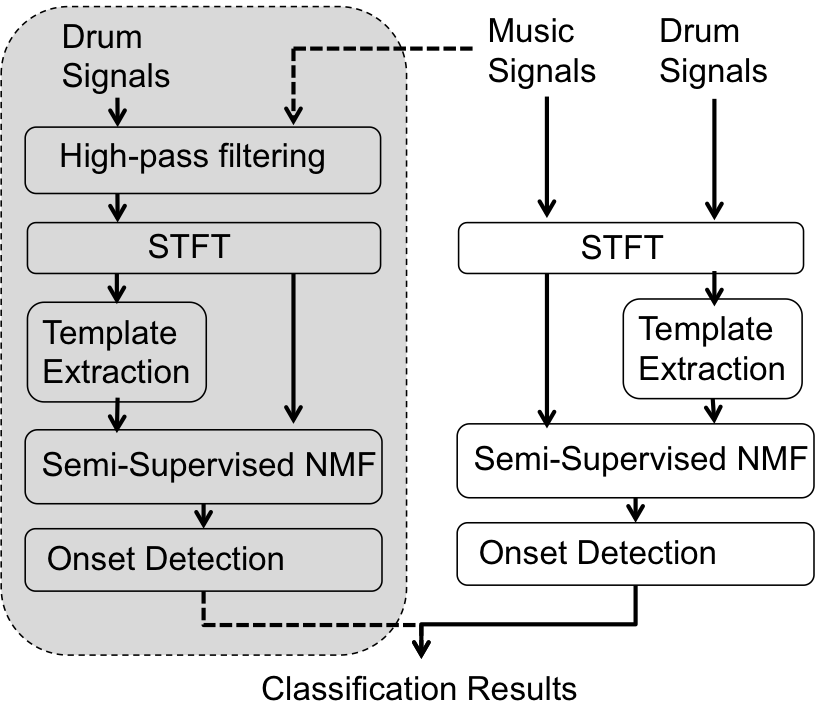
\includegraphics[width=\columnwidth]{flowchart.png}}}
 \caption{Flowchart of the drum transcription system} %SINCE YOU GIVE OTHER FILTER RESULTS AS WELL: WHY DON'T YOU JUST SAY FILTERING INSTEAD OF REFERRING TO THE HP?
 \label{fig:flowchart}
\end{figure}


The following subsections provide more details on the template extraction and activity detection. 


\subsubsection{Template Extraction}\label{subsubsec:template extraction}
As mentioned above, the dictionary matrix $W_D$ is created by extracting a template spectrum from isolated training drum samples. The template magnitude spectrum is median spectrum of all individual events of one drum class in the training set. The length of each event  is approximately \unit[80]{ms}. The templates are extracted for the three classes Hi-Hat (HH), Bass Drum (BD) and Snare Drum (SD).   

\subsubsection{Activity Detection}\label{subsubsec:activity detection}
High activity values in the activation matrix $H_D$ indicate the presence of a drum event. More specifically, the activity difference of each row of the dictionary matrix could be considered as the onset novelty function of each individual drum. We use a median filter as a standard approach to create an adaptive threshold for pick peaking result. 
%I DON'T THINK WE NEED MORE DETAILS HERE --- ESPECIALLY THE EQUATION DOES NOT SEEM NECESSARY.
%The implementation of the median filter is shown in Eq.~\eqref{eq:medianFilter}. The G is the time-varying threshold. Q is a function that extracts the median from previous input signal within a window size = \unit[100]{ms}. Lambda is an offset parameter to control the sensitivity of the threshold.
%% equation here
%\begin{equation}
%G(t) = \lambda + Q(t)
%\label{eq:medianFilter}
%\end{equation}\\

\section{Evaluation}\label{sec:Evaluation}
\subsection{Dataset Description}\label{subsec:data set description}

The experiments have been conducted on the \textit{minus one} subset from the ENST public drum data set (\cite{Gillet2006}). This data set consists of recordings from three different drummers performing on their own drum kits. The set for each drummer contains individual hits, short phrases of drum beats, drum solos, and short excerpts played with the accompaniments. The minus one subset has 64 tracks of polyphonic music. Each track in this subset has a length of approximately \unit[70]{s} with varying style. More specifically, the subset features many drum playing techniques such as ghost notes, flam, and drag; these techniques are considered difficult to identify with existing drum transcription systems. Since we are only interested in the three classes HH, BD, and SD, tracks missing one of these instruments or featuring specific playing techniques have been discarded, leaving a subset of 53 out of 64 tracks.

The accompaniments are mixed with the drum tracks in the data set without any modification (e.g., no level adjustment). The distribution of onset counts per class per drummer is shown in \tabref{tab:onsetCount}. %More details on the creation process of this data set could be found in their corresponding paper.  

The drums template (see Sect.~\ref{subsubsec:template extraction}) have been generated from the tracks with single hits. Each track contains 5 to 6 single hits on different drums. The onset position of these single hits were determined using the annotated ground truth. 
 
%============= Onset event counts in the used tracks
\begin{table}[h]
\begin{center}
\begin{tabular}{|c|c|c|c|c|}
\hline
 & \textbf{Drum.~1}    & \textbf{Drum.~2}    & \textbf{Drum.~3}    & \textbf{Total} \\ \hline
\textbf{HH}        & 1942 & 2145 & 1813 & 5900  \\ \hline
\textbf{BD}        & 2140 & 1488 & 1378 & 5006  \\ \hline
\textbf{SD}        & 2165 & 2079 & 1994 & 6238  \\ \hline
\textbf{Total}     & 6247 & 5712 & 5185 & 17144 \\ \hline
\end{tabular}
 \caption{Onset counts in selected data set}%- IS THIS FOR THE 64 OR THE 53 TRACKS? -- 53!
 \label{tab:onsetCount}
\end{center}
\end{table}

\subsection{Evaluation Procedure}\label{subsec:evaluation procedure}

%In this paper, two different evaluation processes have been performed. The evaluation only focus on transcribing close hihat, snare drum and bass drum, therefore, for tracks that are performed with ride cymbal, open hihat, cross stick..etc, they are excluded in the evaluation process. A subset of 53 out of the 64 tracks are used in the evaluation process. 

We evaluate two different combinations of training and test data. 

First, we use training samples from all three drummers to train the drum basis matrix, and test the system on all $53$ tracks. In this test run, we also evaluate the results in case of filtered training and testing signals. %In addition, two experiments using filters to enhance the performances have been conducted. All the filters are set with a constant cutoff frequency derived from the average spectrum. 

Second, we investigate cross-performer validation as shown in \figref{fig:cross}. The training samples are selected only from one drummer, and the test samples will be only the other drummers' recordings. This scenario should be similar to a real-world use case for which the trained drum sounds are not necessarily similar to the drum sounds in the target signals.
%when a drummer is selected as the source of training data, the trained basis matrix will be constructed only based on his recordings, and will be used to decompose the other drummer’s recordings. This process aims to simulate the real situation, where the drum sounds in the template might be totally different from the sounds in the target signals.

%============= Cross-performer validation figure
\begin{figure}
 \centerline{\framebox{
 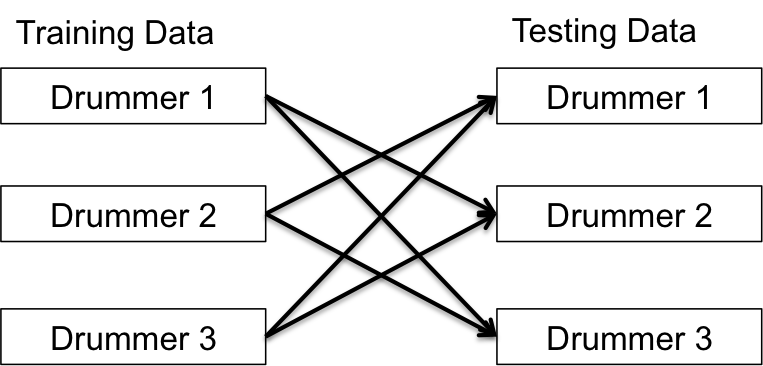
\includegraphics[width=\columnwidth]{cross.png}}}
 \caption{Cross-performer validation process.}
 \label{fig:cross}
\end{figure}

The evaluation metrics follow by the standard calculation of the precision (P), recall (R), and F-measure (F). % as shown in Eq.~\eqref{eq:precision}, Eq.~\eqref{eq:recall} and Eq.~\eqref{eq:Fmeasure}. The $tp$, $fp$, and $fn$ stand for true positive, false positive, and false negative, respectively. 
An onset is considered to be a match with the ground truth if the time deviation between the annotated and detected onset is less or equal to \unit[50]{ms}.  
%\begin{equation}
%Precision = \frac{tp}{tp + fp}
%\label{eq:precision}
%\end{equation}
%
%% equation here
%\begin{equation}
%Recall = \frac{tp}{tp + fn}
%\label{eq:recall}
%\end{equation}
%
%% equation here
%\begin{equation}
%F-measure = \frac{2 \times Precision \times Recall}{Precision + Recall}
%\label{eq:Fmeasure}
%\end{equation}
  



\subsection{Evaluation Results}\label{subsec:evaluation results}

\subsubsection{Pre-Evaluation Test}
In an initial test to determine the rank $r_H$ of the algorithm, $r_H = {5, 10, 20, 40, 80, 160, 320}$ have been tested. The resulting individual F-measures are shown in \figref{fig:rankTest}. A general trend of decreasing performance with increasing $r_H$ can be observed, especially for lower frequency sounds such as SD and BD. Based on this observation, a rank number $r_H = 10$ is chosen in current setup. %SO IS THIS THE OVERALL RANK HERE OR ONLY THE HARMONIC RANK?

%============= Rank Test Figure
\begin{figure}
 \centerline{\framebox{
 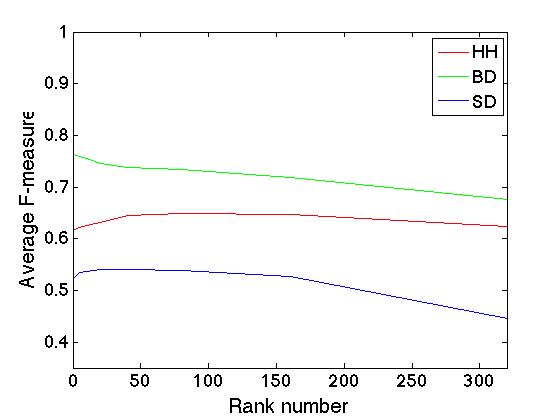
\includegraphics[width=\columnwidth]{rankTest.png}}}
 \caption{Average F-measure versus NMF rank}%WHY NOT ADD A GRID AND MAYBE INCREASE LINE THICKNESS?
 \label{fig:rankTest}
\end{figure}

\subsubsection{Evaluation I}
\tabref{tab:basicResults} shows the results (precision, recall, and F-measure) when using the complete training and test set. 
The results for the standard setup (the white section of \figref{fig:flowchart}) are given in the column named \textit{Standard}. The middle column (\textit{HPF+LPF+BPF}) presents the results for signals pre-processed with filters. More specifically, we use three filters corresponding to the three instruments we intend to detect; the filter frequencies are derived from the median magnitude spectra: 
\begin{itemize}
    \item   HH: $f_{hp} = \unit[8000]{Hz}$
    \item   SD: $f_{bp} = \unit[200--500]{Hz}$
    \item   BD: $f_{lp} = \unit[150]{Hz}$
\end{itemize}
The last column uses a similar setup, but only one high-pass filter for the HH class.

%============= Train on All templates
\begin{table}[h]
\begin{center}
\begin{tabular}{|c|c|c|c|c|}
\hline
\multicolumn{2}{|c|}{}  & Standard & HPF+LPF+BPF & HPF only \\ \hline
\multirow{3}{*}{HH} & P & 0.605    & 0.671       & 0.675    \\ \cline{2-5} 
                    & R & 0.713    & 0.737       & 0.736    \\ \cline{2-5} 
                    & F & 0.654    & 0.702       & \textbf{0.704}    \\ \hline
\multirow{3}{*}{BD} & P & 0.723    & 0.662       & 0.740    \\ \cline{2-5} 
                    & R & 0.837    & 0.855       & 0.839    \\ \cline{2-5} 
                    & F & 0.776    & 0.746       & \textbf{0.786}    \\ \hline
\multirow{3}{*}{SD} & P & 0.678    & 0.591       & 0.676    \\ \cline{2-5} 
                    & R & 0.566    & 0.583       & 0.569    \\ \cline{2-5} 
                    & F & 0.617    & 0.587       & \textbf{0.618}    \\ \hline
\end{tabular}
\end{center}
 \caption{Transcription results using all training templates} % I DONT UNDERSTAND WHY THE BD RESULTS INCREASE FOR HPF ONLY. I THOUGHT THE BD WAS PROCESSED ON THE UNMODIFIED SIGNAL THEN?
 \label{tab:basicResults}
\end{table}

It can be observed that using the filters does not necessarily improve the results. The combination of three filters in particular seems to improve results slightly for HH, but the drop in precision of the other classes results in a lower F-measure. In the third, high-pass-only, case we can identify a general trend for improved results in all classes, although the increase for SD and especially BD is rather negligible. These small increase might due the random initialization of the harmonic dictionary, but the deviations are not significant.   
%COMPARE OVERALL RESULTS WITH (THE) OTHER PUBLICATION(S).
Comparing with the reported F-measure of 77.7\%, 65.0\% and 64.8\% for HH, BD and SD in \cite{Gillet2008}, our results show better performance on BD, but slightly worse performance in SD and HH. However, in our method, the training process require less amount of training data to achieve the results at same level, which could potential provide a better use case for a more generic drum transcription system.     

The results in the middle column of \tabref{tab:basicResults} indicate that by filtering the templates and signals with constant cutoff frequencies, the performance of BD and SD drop slightly.	Some possible reasons might contribute to this result. First, although the filtering process could suppress contents in the unwanted frequency bins, it also could remove many information that might help to differentiate instruments such as BD and Bass Guitar. Second, in current parameter settings, the band-pass and low-pass filtered signals might only have few bins to represent the spectrum, which might increase the difficulty for the semi-NMF to adapt. Third, when the signals are filtered, the current rank setting $r_H$ might not be optimal for the task.  

%WHY MIGHT THE FILTERED RESULTS BE WORSE? SPECULATE ON DIFFERENT INSTRUMENT/PLAYER CHARACTERETICS, SPECTRAL RESOLUTION, ...
%
%COMPARE INTER-INSTRUMENT RESULTS.
%
%IS THE RELATION OF RECALL AND PRECISION WORTH DISCUSSING?
%
%WHAT ELSE CAN BE DISCUSSED HERE< WHAT ELSE CAN WE LEARN FROM THE RESULTS.

%There are three experiment setups using the same training data and testing data as mentioned in \ref{subsec:evaluation procedure}. In the first setup, the original signals of the drum samples are used to train the basis matrix, and the original signals from the minus one subset are used as the target signals. The results show that the average F-measure for HH, BD and SD are 0.654, 0.776 and 0.617 respectively. A second setup uses three different filters to pre-process the extracted templates as well as the target signals. A high-pass filter with $f_{hp} = \unit[8000]{Hz}$ is used for HH; a band-pass filter with $f_{bp} = \unit[200--500]{Hz}$ is used for SD; a low-pass filter with $f_{sd} = \unit[150]{Hz}$ is used for BD. The results show that the performance for HH has a significant improvement of 0.702, but the performance for BD and SD drop slightly. Finally, a setup uses only high-pass filter to retain the best overall results has been settled in the current implementation. 

\subsubsection{Evaluation II}
LETS THINK OF WAYS TO CUMMARIZE THESE THREE TABLES IN ONE TABLE AND A GRAPH, MAYBE DISCARDED PRECISION AND RECALL. MAYBE ALSO OVERALL AVERAGE MEASURES (TRAINING WITH 1, TESTING WITH ALL)?

In order to investigate the dependency of our approach with respect to the similarity of training and test drum sounds, we conduct a cross-performer evaluation as shown in \figref{fig:cross}. No filters have been applied during the process. There results are listed in \tabref{tab:trainDr1}, \tabref{tab:trainDr2}, and \tabref{tab:trainDr3}.

%============= Train on Drummer 1 templates
\begin{table}[h]
\begin{center}
\begin{tabular}{|c|c|c|c|c|}
\hline
\multicolumn{2}{|c}{Training} & \multicolumn{3}{|c|}{Drummer 1}   \\ \hline
\multicolumn{2}{|c|}{Testing} & Drummer 1 & Drummer 2 & Drummer 3 \\ \hline
\multirow{3}{*}{HH}    & P    & 0.662     & 0.621     & 0.564     \\ \cline{2-5} 
                       & R    & 0.670     & 0.749     & 0.692     \\ \cline{2-5} 
                       & F    & 0.666     & \textbf{0.679}     & 0.622     \\ \hline
\multirow{3}{*}{BD}    & P    & 0.620     & 0.781     & 0.850      \\ \cline{2-5} 
                       & R    & 0.393     & 0.914     & 0.900      \\ \cline{2-5} 
                       & F    & 0.481     & 0.842     & \textbf{0.874}     \\ \hline
\multirow{3}{*}{SD}    & P    & 0.639     & 0.800     & 0.589     \\ \cline{2-5} 
                       & R    & 0.546     & 0.608     & 0.487     \\ \cline{2-5} 
                       & F    & 0.588     & \textbf{0.691}     & 0.533     \\ \hline
\end{tabular}
 \caption{Transcription results using drummer 1 training templates.}
 \label{tab:trainDr1}
\end{center}
\end{table}

%============= Train on Drummer 2 templates
\begin{table}[h]
\begin{center}
\begin{tabular}{|c|c|c|c|c|}
\hline
\multicolumn{2}{|c}{Training} & \multicolumn{3}{|c|}{Drummer 2}   \\ \hline
\multicolumn{2}{|c|}{Testing} & Drummer 1 & Drummer 2 & Drummer 3 \\ \hline
\multirow{3}{*}{HH}    & P    & 0.661     & 0.600     & 0.541     \\ \cline{2-5} 
                       & R    & 0.667     & 0.787     & 0.699     \\ \cline{2-5} 
                       & F    & 0.664     & \textbf{0.681}     & 0.610     \\ \hline
\multirow{3}{*}{BD}    & P    & 0.466     & 0.846     & 0.699     \\ \cline{2-5} 
                       & R    & 0.603     & 0.986     & 0.854     \\ \cline{2-5} 
                       & F    & 0.525     & \textbf{0.910}     & 0.769     \\ \hline
\multirow{3}{*}{SD}    & P    & 0.625     & 0.849     & 0.529     \\ \cline{2-5} 
                       & R    & 0.550     & 0.624     & 0.486     \\ \cline{2-5} 
                       & F    & 0.585     & \textbf{0.719}     & 0.506     \\ \hline
\end{tabular}
 \caption{Transcription results using drummer 2 training templates.}
 \label{tab:trainDr2}
\end{center}
\end{table}

%============= Train on Drummer 3 templates
\begin{table}[h]
\begin{center}
\begin{tabular}{|c|c|c|c|c|}
\hline
\multicolumn{2}{|c}{Training} & \multicolumn{3}{|c|}{Drummer 3}   \\ \hline
\multicolumn{2}{|c|}{Testing} & Drummer 1 & Drummer 2 & Drummer 3 \\ \hline
\multirow{3}{*}{HH}    & P    & 0.614     & 0.599     & 0.523     \\ \cline{2-5} 
                       & R    & 0.660     & 0.717     & 0.675     \\ \cline{2-5} 
                       & F    & 0.636     & \textbf{0.652}     & 0.589     \\ \hline
\multirow{3}{*}{BD}    & P    & 0.506     & 0.862     & 0.800     \\ \cline{2-5} 
                       & R    & 0.636     & 0.965     & 0.932     \\ \cline{2-5} 
                       & F    & 0.564     & \textbf{0.910}     & 0.861     \\ \hline
\multirow{3}{*}{SD}    & P    & 0.477     & 0.615     & 0.564     \\ \cline{2-5} 
                       & R    & 0.580     & 0.598     & 0.534     \\ \cline{2-5} 
                       & F    & 0.523     & \textbf{0.607}     & 0.548     \\ \hline
\end{tabular}
 \caption{Transcription results using drummer 3 training templates.}
 \label{tab:trainDr3}
\end{center}
\end{table}

The results show a simple trend: the test set featuring drummer 2 give nearly always the best results, regardless of the training set. The Bass Drum of drummer 2 seems to be particularly easy to detect. An even more surprising result is that there does not seem to be an obvious increase of the F-measure when the training drummer and test set drummer are identical.
These results indicate that this algorithm is relatively robust against differences between the drum template and the sound of the drum to be detected. This would allow to construct a template from different sound sources independent of the recording to be analyzed allowing far more general applications. However, the performance of this setup still needs to be confirmed with a cross-data set validation.

%ANYTHING ELSE TO DISCUSS HERE?

%Although this process focuses on the exclusiveness between the players, the results of training and testing on the same drummer are still reported in \tabref{tab:trainDr1}, \tabref{tab:trainDr2} and \tabref{tab:trainDr3}. No filters have been applied during the process. In \tabref{tab:trainDr1}, the drum basis matrix is trained on recordings of drummer 1 only. The matrix is then used to decompose polyphonic recordings of different drummers and transcribe drum events. As shown in the table, the testing data from drummer 2 has the best average F-measures of 0.679, 0.842, and 0.691 for HH, BD, and SD.   

%In \tabref{tab:trainDr2}, the drum basis matrix is trained on recordings of drummer 2 only. As shown in the table, the testing data from drummer 2 has the best average F-measures of 0.846, 0.910, and 0.719 for HH, BD, and SD. However, since the basis matrix is trained on the recordings of drummer 2, an improvement of the performance on the same drummer's recording is expected. As for the other drummers, the performance is within the same range.     

%Finally, in \tabref{tab:trainDr3}, the drum basis matrix is trained on recordings of drummer 3 only. As shown in the table, the testing data from drummer 2 has the best average F-measures of 0.862, 0.910, and 0.607 for HH, BD, and SD. In general, the testing data from drummer 2 has the best overall performance with different training data from all the drummers. Besides, all the results have a similar trend no matter which training data is used. This result might imply that this algorithm is less template dependent, allowing a general use case where a drum template could be constructed from different sound sources and be applied to different polyphonic recordings. However, the performance of this setup still needs to be confirmed with a cross-data set validation.      

\section{Conclusion}\label{sec:Conclusion}

We have presented a drum transcription system for polyphonic music using semi-supervised NMF. This method uses a pre-trained dictionary matrix to decompose the target signal and extract the activation matrix. This evaluation results show that this method is able to achieve 61~77\% accuracy in polyphonic music. 
It has the following advantages: 
First, simultaneous sounds can be detected separately. Traditional systems for drum detection often have difficulties with simultaneous events, especially when the number of instruments increases. %Normally, when more classes of drums are being considered in a instance-based transcription task, more combination of classes need to be considered, and the situation could be more complicated. With a NMF approach, there is no need to train more classes to handle such situations. 
Second, adjustment of the parameter $r_H$ allows the algorithm to adapt to different different types of polyphonic music. 
Third, cross-perfomer evaluation results indicate a robustness against template mismatches, possibly allowing the application in situations with minimum prior knowledge. %Furthermore, the results from the cross-performer validation indicate that this method still apply to the situations when minimum prior knowledge about the drum sounds in the target signal is given.
Fourth, the approach requires only trivial extensions to be able to be used as a drum separation system.
Last but not least, the approach only requires a few drum samples to train the dictionary matrix, and the evaluation results indicate that the performance is comparable with the existing methods. This means the current approach has less constraints on the user input data, and could potentially be realized as a generic drum transcription system .

%FUTURE WORK: ADD HERE WHAT YOU MIGHT WANT TO DO SPECIFICALLY (WHAT YOU PLAN TO DO) AND MORE GENERAL DIRECTIONS.
There are some possible directions for the future works: first of all, a comparison between this approach with Probabilistic Latent Component Analysis (PLCA) and looking for means to adapt the template during the decomposition might be a way to further generalize the current method. Also, other distance metrics such as KL-divergence or beta divergence could be implemented for better approximations. Finally, finding a method to automatically determine the rank $r_H$ could optimize this approach against different polyphonic music. To achieve a complete drum transcription system in polyphonic music, however, more factors such as playing techniques and different drum setups still need to be addressed in the future. 

%Dummycite: \cite{tzanetakis_musical_2002}

%\section{Reference}
%
%
%% I haven't done this part yet...
%
%
%
%%============= This part is for reference only, will be removed once my parts are finished =============
%\section{Equations}
%
%Equations should be placed on separated lines and numbered.
%The number should be on the right side, in parentheses.
%
%\begin{equation}
%E=mc^{2}
%\end{equation}

%\section{Citations}
%
%All bibliographical references should be listed at the end,
%inside a section named ``REFERENCES,'' numbered and in alphabetical order.
%Also, all references listed should be cited in the text.
%When referring to a document, type the numbering square brackets
%\cite{Author:00} or \cite{Author:00,Someone:10,Someone:04}.
%
%\begin{thebibliography}{citations}
%
%\bibitem {Author:00}
%E. Author:
%``The Title of the Conference Paper,''
%{\it Proceedings of the International Symposium
%on Music Information Retrieval}, pp.~000--111, 2000.
%
%\bibitem{Someone:10}
%A. Someone, B. Someone, and C. Someone:
%``The Title of the Journal Paper,''
%{\it Journal of New Music Research},
%Vol.~A, No.~B, pp.~111--222, 2010.
%
%\bibitem{Someone:04} X. Someone and Y. Someone: {\it Title of the Book},
    %Editorial Acme, Porto, 2012.
%
%\end{thebibliography}
\bibliographystyle{ismir2014}
\bibliography{cwIsmirRef}
%\bibliography{ismir2014template}

\end{document}
